\documentclass[systeme]{compas2026}
\usepackage{hyperref}
\usepackage{booktabs}
\usepackage{tabularx}
\usepackage{algorithm}
\usepackage{algpseudocode}
\usepackage{enumitem}
\usepackage{tikz}
\usetikzlibrary{positioning, arrows.meta, shapes.geometric, calc, fit}

\toappear{1}

\newcommand{\cmark}{\ding{51}}
\newcommand{\xmark}{\ding{55}}

% Commandes utiles
\newcommand{\todo}[1]{\textcolor{red}{\textbf{[TODO: #1]}}}

\title{Heuristique, CSP ou LLM ? Étude comparative du coût énergétique du placement de services multi-composants dans le Cloud}

\author{Théo Hardy$^{1}$, Farah Aït-Salaht$^{1}$}
\address{$^{1}$De Vinci Higher Education, De Vinci Research Center, Paris La Défense, France
theo.hardy@edu.devinci.fr}

\date{}

\begin{document}

\maketitle

% ============================================================
%  RÉSUMÉ
% ============================================================
\begin{abstract}
Le placement de services multi-composants sur une infrastructure Cloud hétérogène pose un défi d'optimisation combinant satisfaction de contraintes (CPU, RAM, bande passante, latence bout-en-bout) et minimisation de divers objectifs tels que le coût, la latence ou la consommation énergétique. Si les approches heuristiques et exactes sont bien étudiées, l'émergence des grands modèles de langage (LLM) comme outils de résolution de problèmes combinatoires ouvre une voie nouvelle et peu explorée.

Dans cet article, nous formalisons le problème de placement d'une application de type \emph{Data Stream Processing} (DSP) multi-composants sur des machines virtuelles hétérogènes et géo-distribuées, et nous \emph{évaluons l'empreinte énergétique} des solutions produites par trois paradigmes de résolution distincts. Nous considérons un déploiement réel sur Google Cloud Platform (GCP) comme cas d'étude. Les trois approches comparées sont~: (i)~une heuristique gloutonne \emph{First Fit Decreasing} (FFD), (ii)~un solveur exact par programmation par contraintes (CSP via OR-Tools), et (iii)~une approche LLM-as-Solver dans laquelle un modèle de langage (GPT-4o et Llama~3 via Ollama) reçoit une description structurée du problème et renvoie directement un placement. La consommation énergétique de chaque placement est estimée à l'aide d'un modèle linéaire fondé sur l'utilisation CPU, largement adopté dans la littérature.

Nos résultats expérimentaux montrent que \todo{résumé des résultats clés~: qualité relative des 3 approches, écart énergétique, temps de résolution, coût du LLM}. Nous discutons les implications pratiques de l'utilisation des LLM comme solveurs, notamment leur non-déterminisme, leur coût énergétique propre, et les scénarios où ils constituent une alternative viable.
\end{abstract}

\smallskip
\noindent\textbf{Mots-clés :} Placement de services, Data Stream Processing, consommation énergétique, programmation par contraintes, LLM, Cloud Computing

% ============================================================
%  1. INTRODUCTION
% ============================================================
\section{Introduction}
\label{sec:intro}

Le Cloud Computing offre des ressources élastiques mais hétérogènes, réparties dans des régions et zones géographiques distinctes. Le déploiement d'applications orientées service, composées de plusieurs processus communicants, nécessite de décider \emph{quel composant placer sur quel nœud}, en respectant des contraintes de capacité (CPU, RAM), de réseau (bande passante, latence bout-en-bout) et de qualité de service. Ce problème de placement, NP-difficile~\cite{wang2020service}, a des conséquences directes sur de multiples objectifs d'optimisation~: coût financier, latence applicative, mais aussi consommation énergétique. Un placement qui fragmente les composants entre régions distantes augmente le trafic réseau, sollicite la bande passante inter-régions et mobilise des nœuds sous-optimaux, entraînant une surconsommation énergétique.

Traditionnellement, deux familles d'approches dominent la littérature : les \emph{heuristiques} (First Fit, Best Fit, algorithmes génétiques), rapides mais sans garantie d'optimalité, et les \emph{méthodes exactes} (programmation linéaire, CSP, ILP), optimales mais limitées en passage à l'échelle~\cite{mann2015allocation}. Récemment, les grands modèles de langage (LLM) ont démontré des capacités surprenantes de raisonnement sur des problèmes combinatoires~\cite{yang2024large}, ouvrant la question de leur utilisation comme solveurs de placement.

\smallskip
Dans cet article, nous nous intéressons spécifiquement à la \emph{consommation énergétique} comme critère d'évaluation des placements. Nous proposons une étude comparative de trois paradigmes appliqués au placement d'une application de type \emph{Data Stream Processing} (DSP) multi-composants sur des machines virtuelles hétérogènes et géo-distribuées~: comment ces approches se comportent-elles en termes d'énergie consommée, de respect des contraintes et de coût de résolution~? Nos contributions sont les suivantes~:
\begin{enumerate}[leftmargin=*, nosep]
    \item La \textbf{formalisation} du problème de placement multi-composant avec un modèle énergétique linéaire fondé sur l'utilisation CPU~\cite{beloglazov2012energy}, servant de base commune pour comparer les approches.
    \item La \textbf{comparaison expérimentale} de trois approches (FFD, CSP, LLM-as-Solver) sur une infrastructure Cloud réelle (Google Cloud Platform), évaluant qualité du placement, énergie estimée, temps de résolution et respect des contraintes.
    \item L'\textbf{évaluation du coût du solveur} lui-même~: temps de calcul pour FFD/CSP, coût en tokens et énergie d'inférence estimée pour les LLM (GPT-4o distant vs.\ Llama~3 local via Ollama).
\end{enumerate}

% ============================================================
%  2. MODÈLE DU SYSTÈME
% ============================================================
\section{Modèle du système}
\label{sec:model}

\subsection{Application DSP multi-composants}

Nous considérons une application de type \emph{Data Stream Processing} (DSP), dans laquelle un flux continu de données est traité par un pipeline de composants. L'application est modélisée comme un graphe orienté $G_a = (S, L)$ où $S = \{s_0, s_1, \ldots, s_K\}$ est l'ensemble des composants et $L \subseteq S \times S$ l'ensemble des flux de communication. Le composant $s_0$ représente la \emph{source de données} (point d'entrée du pipeline, e.g., un flux de capteurs ou un broker de messages). Les composants $s_1, \ldots, s_K$ constituent les opérateurs de traitement. Chaque composant $s_i$ ($i \geq 1$) a des besoins~:
\begin{itemize}[nosep]
    \item $\psi_i^{cpu}$ : demande CPU (en vCPU ou millicores),
    \item $\psi_i^{ram}$ : demande mémoire (en Mo),
    \item $\lambda_i$ : taux de requêtes en entrée (req/s) pour le workload.
\end{itemize}
Chaque flux $(s_i, s_j) \in L$ est caractérisé par un débit de données $d_{ij}$ (Mo/s) et consomme de la bande passante sur le lien réseau entre les nœuds hébergeant $s_i$ et $s_j$. L'application impose une contrainte de latence bout-en-bout $\mathcal{L}_{max}$ entre la source $s_0$ et le dernier opérateur du pipeline.

\begin{figure}[H]
    \centering
    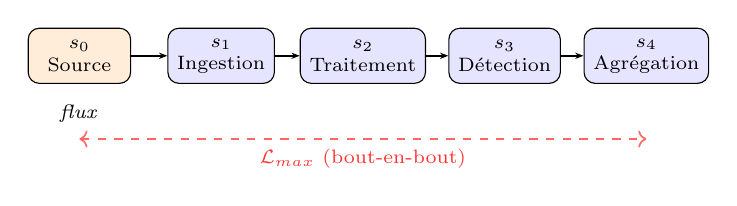
\begin{tikzpicture}[
        node distance=1.8cm,
        svc/.style={
            draw, rounded corners, fill=blue!10,
            minimum width=1.3cm, minimum height=0.7cm,
            font=\scriptsize, align=center
        },
        src/.style={
            draw, rounded corners, fill=orange!15,
            minimum width=1.3cm, minimum height=0.7cm,
            font=\scriptsize, align=center
        },
        arr/.style={-{Stealth[length=3pt]}, line width=0.6pt}
    ]
    \node[src] (s0) {$s_0$\\Source};
    \node[svc, right of=s0] (s1) {$s_1$\\Ingestion};
    \node[svc, right of=s1] (s2) {$s_2$\\Traitement};
    \node[svc, right of=s2] (s3) {$s_3$\\Détection};
    \node[svc, right of=s3] (s4) {$s_4$\\Agrégation};

    \draw[arr] (s0) -- (s1);
    \draw[arr] (s1) -- (s2);
    \draw[arr] (s2) -- (s3);
    \draw[arr] (s3) -- (s4);

    \node[font=\scriptsize, below=0.15cm of s0] {\emph{flux}};

    % Latence bout-en-bout
    \draw[<->, dashed, red!60, line width=0.6pt]
      ([yshift=-0.7cm]s0.south) -- ([yshift=-0.7cm]s4.south)
      node[midway, below, font=\scriptsize, red!80] {$\mathcal{L}_{max}$ (bout-en-bout)};
    \end{tikzpicture}
    \caption{Graphe applicatif DSP~: source de données $s_0$ et pipeline à 4~opérateurs avec flux de données et contrainte de latence bout-en-bout.}
    \label{fig:app_graph}
\end{figure}

\subsection{Infrastructure physique}

L'infrastructure est modélisée comme un graphe $G_p = (V, E)$ où $V = \{v_1, \ldots, v_N\}$ est l'ensemble des machines virtuelles (VMs) et $E$ les liens réseau. Chaque VM $v_j$ dispose de~:
\begin{itemize}[nosep]
    \item $C_j^{cpu}$ : capacité CPU disponible (vCPU),
    \item $C_j^{ram}$ : capacité mémoire (Mo),
    \item $P_{idle,j}$, $P_{max,j}$ : puissance au repos et à pleine charge (W),
    \item $r_j$ : zone de déploiement (e.g., région géographique).
\end{itemize}
Chaque lien $(v_j, v_k) \in E$ est caractérisé par une latence mesurée $\ell_{jk}$ (ms) et une bande passante $\mathcal{B}_{jk}$ (Mbps). La bande passante constitue une contrainte importante~: un flux $d_{ij}$ entre deux composants placés sur des VMs distantes ne peut excéder $\mathcal{B}_{\pi(s_i),\pi(s_j)}$. Les latences intra-zone, inter-zone et inter-région sont mesurées empiriquement.

\smallskip
\noindent\textbf{Cas d'étude~: Google Cloud Platform.}
Dans ce travail, nous instancions cette modélisation sur des VMs Google Compute Engine (GCE) de types hétérogènes, réparties dans plusieurs zones et régions (\ref{tab:vms}). Ce choix est motivé par la disponibilité de types de machines variés (familles e2, n2) et par la possibilité de mesurer les latences et bandes passantes inter-zones de manière empirique (\ref{sec:setup}).

\begin{table}[t]
    \centering
    \footnotesize
    \caption{VMs GCE utilisées dans le cas d'étude (instances SPOT hétérogènes)}
    \label{tab:vms}
    \begin{tabularx}{\columnwidth}{l X c c c}
        \toprule
        \textbf{VM} & \textbf{Type GCE} & \textbf{vCPU} & \textbf{RAM (Go)} & \textbf{Zone} \\
        \midrule
        $v_0$ & n2-standard-4 & 4 & 16 & europe-west4-a \\
        $v_1$ & e2-standard-2 & 2 &  8 & europe-west9-a \\
        $v_2$ & e2-medium     & 2 &  4 & europe-west9-b \\
        $v_3$ & e2-small      & 1 &  2 & europe-west9-c \\
        $v_4$ & e2-micro      & 1 &  1 & europe-west9-a \\
        \bottomrule
    \end{tabularx}
\end{table}

\subsection{Problème de placement}

Un placement est une fonction $\pi : S \rightarrow V$ qui assigne chaque composant $s_i$ ($i \geq 1$) à une VM $v_j$. Un placement est \emph{valide} s'il respecte~:
\begin{align}
    \sum_{s_i : \pi(s_i)=v_j} \psi_i^{cpu} &\leq C_j^{cpu} \quad \forall\, v_j \in V \label{eq:cst_cpu} \\
    \sum_{s_i : \pi(s_i)=v_j} \psi_i^{ram} &\leq C_j^{ram} \quad \forall\, v_j \in V \label{eq:cst_ram} \\
    d_{ik} &\leq \mathcal{B}_{\pi(s_i),\pi(s_k)} \quad \forall\, (s_i, s_k) \in L \label{eq:cst_bw} \\
    \sum_{(s_i, s_j) \in \text{chemin}} \ell_{\pi(s_i), \pi(s_j)} &\leq \mathcal{L}_{max} \label{eq:cst_latency}
\end{align}

\subsection{Modèle énergétique}
\label{subsec:energy_model}

Nous adoptons le modèle linéaire fondé sur l'utilisation CPU, initialement proposé par Beloglazov et al.~\cite{beloglazov2012energy} et largement repris dans la littérature sur le placement de services~:
\begin{equation}\label{eq:power}
    P_j(u_j) = P_{idle,j} + (P_{max,j} - P_{idle,j}) \cdot u_j
\end{equation}
où $u_j \in [0,1]$ est le taux d'utilisation CPU de la VM $v_j$, résultant du placement~:
\begin{equation}\label{eq:util}
    u_j = \frac{\sum_{s_i : \pi(s_i) = v_j} \psi_i^{cpu}}{C_j^{cpu}}
\end{equation}

%L'énergie totale du système sur une période $T$ est~:
%\begin{equation}\label{eq:energy_total}
%    E_{total}(\pi) = \underbrace{\sum_{v_j \in V^{act}} P_j(u_j) \cdot T}_{E_{compute}} + \underbrace{\sum_{(s_i,s_k) \in L} E_{net}(i,k,\pi)}_{E_{network}}
%\end{equation}
%où $V^{act} = \{v_j \mid \exists\, s_i,\, \pi(s_i) = v_j\}$ est l'ensemble des VMs actives. 
%L'énergie réseau $E_{net}$ est proportionnelle au volume de données transmis entre composants placés sur des VMs distinctes~:
%\begin{equation}\label{eq:energy_net}
%    E_{net}(i,k,\pi) = \begin{cases}
%        0 & \text{si } \pi(s_i) = \pi(s_k) \\
%        P_{tx} \cdot \dfrac{d_{ik}}{\mathcal{B}_{\pi(s_i),\pi(s_k)}} \cdot T & \text{sinon}
%    \end{cases}
%\end{equation}

%\textbf{Critère d'évaluation énergétique~:} Pour chaque placement $\pi$ valide, nous calculons $E_{total}(\pi)$ selon~\eqref{eq:energy_total}. Le CSP utilise cette quantité comme fonction objectif à minimiser, tandis que pour FFD et le LLM, $E_{total}$ sert de métrique a~posteriori permettant de comparer la qualité énergétique des solutions produites.

\smallskip
\noindent\textbf{Justification du choix de modèle.}
Parmi les formulations existantes dans la littérature~\cite{beloglazov2012energy, iftikhar2023hunterplus, adhikari2019energy}, le modèle linéaire (\ref{eq:power}) est retenu pour trois raisons~: (i)~il est le plus répandu (adopté par la majorité des travaux de placement dans le Cloud et le continuum), (ii)~il ne requiert que deux paramètres par nœud ($P_{idle}$, $P_{max}$) calibrables via \texttt{stress-ng} + monitoring, et (iii)~il est suffisamment expressif pour capturer les différences entre types de VMs hétérogènes. Les modèles non-linéaires (quadratiques) et à base de DVFS sont discutés en \ref{sec:discussion} comme alternatives.


% ============================================================
%  3. APPROCHES DE PLACEMENT
% ============================================================
\section{Approches de placement}
\label{sec:approaches}

\subsection{First Fit Decreasing (FFD), Heuristique}

L'heuristique FFD trie les composants par demande CPU décroissante et les place séquentiellement sur la première VM ayant une capacité suffisante et dont les liens réseau satisfont les contraintes de bande passante. Si la contrainte de latence bout-en-bout est violée, un mécanisme de \emph{backtracking} local tente de rapprocher les composants communicants.

\begin{algorithm}[t]
\caption{First Fit Decreasing (FFD)}
\label{alg:ffd}
\footnotesize
\begin{algorithmic}[1]
\Require $S$ trié par $\psi_i^{cpu}$ décroissant, $V$, $\mathcal{L}_{max}$
\Ensure Placement $\pi$ ou $\varnothing$ si infaisable
\For{chaque composant $s_i \in S$}
    \For{chaque VM $v_j \in V$}
        \If{$\psi_i^{cpu} \leq C_j^{cpu} - \text{alloc}(v_j)$ \textbf{et} $\psi_i^{ram} \leq C_j^{ram} - \text{alloc\_ram}(v_j)$}
            \State $\pi(s_i) \leftarrow v_j$
            \If{$\text{latence\_bout\_en\_bout}(\pi) \leq \mathcal{L}_{max}$}
                \State \textbf{break}
            \Else
                \State annuler $\pi(s_i)$ ; \textbf{continue}
            \EndIf
        \EndIf
    \EndFor
\EndFor
\State \Return $\pi$
\end{algorithmic}
\end{algorithm}

\emph{Complexité~:} $\mathcal{O}(K \cdot N)$ avec $K = |S|$ composants et $N = |V|$ VMs. L'avantage est un temps de résolution quasi-instantané ; la limite est l'absence de garantie d'optimalité.



\subsection{LLM-as-Solver, Approche émergente}
\label{subsec:llm}

Nous utilisons deux LLM comme solveurs directs~:
\begin{itemize}[nosep]
    \item \textbf{GPT-4o}~: modèle commercial (API OpenAI), exécution distante.
    \item \textbf{Llama~3 (8B)}~: modèle open-source exécuté localement via Ollama.
\end{itemize}

\subsubsection{Conception du prompt}

Le LLM reçoit un prompt structuré contenant~: (i)~la description formelle de l'infrastructure (VMs, capacités, zones, latences), (ii)~le graphe applicatif (composants, besoins, flux), (iii)~les contraintes à respecter, et (iv)~le modèle énergétique avec l'instruction de proposer un placement qui minimise la consommation. Le prompt demande une réponse au format JSON strictement structuré~:

\begin{verbatim}
{
  "placement": {
    "s1": "v2",
    "s2": "v2",
    "s3": "v5",
    "s4": "v5"
  },
  "reasoning": "..."
}
\end{verbatim}

\subsubsection{Protocole de non-déterminisme}

Les LLM étant non-déterministes, chaque instance est soumise $R = 10$ fois (température $\tau = 0$ pour GPT-4o, $\tau = 0.1$ pour Llama~3). Nous rapportons la solution médiane, le meilleur cas et la variance. Le prompt est identique pour tous les runs et tous les modèles (\emph{pas de cherry-picking}).

\subsubsection{Coût du solveur}

Un aspect original de notre évaluation est la mesure du \emph{coût de la décision de placement}~:
\begin{itemize}[nosep]
    \item \textbf{FFD~:} temps CPU local (millisecondes).
    \item \textbf{CSP~:} temps CPU du solveur OR-Tools (millisecondes à secondes).
    \item \textbf{GPT-4o~:} nombre de tokens (entrée + sortie), temps de réponse API, coût financier estimé (\$), et énergie d'inférence estimée via les facteurs de~\cite{luccioni2023power}.
    \item \textbf{Llama~3 local~:} temps d'inférence, utilisation CPU/GPU, énergie mesurée localement (via \texttt{powermetrics} ou \texttt{nvidia-smi}).
\end{itemize}


% ============================================================
%  4. PROTOCOLE EXPÉRIMENTAL
% ============================================================
\section{Protocole expérimental}
\label{sec:setup}

\subsection{Application et infrastructure}

\paragraph{Application DSP.}
Nous évaluons le placement d'un pipeline DSP à 4~composants communicants
(Figure~\ref{fig:app_graph})~: $s_0$~(source, 1~vCPU, 1~Go~RAM, flux~400~req/s),
$s_1$~(pré-traitement, 1~vCPU, 1~Go), $s_2$~(traitement, 2~vCPU, 2~Go),
$s_3$~(agrégation, 2~vCPU, 2~Go). Chaque flux de communication est dimensionné à
400~Mbps. Une contrainte de localité (\emph{DZ}) impose le placement de $s_0$ sur le
nœud $v_2$ (zone \texttt{europe-west9-b}), simulant une source de données IoT
territorialement contrainte.

\paragraph{Infrastructure GCP.}
L'infrastructure repose sur $N{=}5$~VMs Google Compute Engine de types
hétérogènes (Table~\ref{tab:vms}), provisionnées comme instances préemptibles
(\emph{SPOT}) via un automate de déploiement idempotent qui associe chaque profil
(CPU,~RAM) à un type GCE, crée les règles réseau nécessaires, puis instancie les
VMs à partir d'un fichier \texttt{.properties}. La topologie à deux niveaux couvre 2~régions et
4~zones~: $v_0$ (\texttt{europe-west4-a}) constitue le niveau Cloud, $v_1$--$v_4$
le niveau Fog/Edge dans \texttt{europe-west9}. Le lien $v_0$--$v_1$ est un lien
inter-région 1~Gbps à 40~ms~; les liens $v_1$--$v_{2,3,4}$ sont des liens
intra-région 500~Mbps à 2~ms. Un nœud dédié \texttt{storm-nimbus}
(\texttt{e2-medium}, \texttt{europe-west9-a}) héberge Apache Storm~2.8.3
(Nimbus\,+\,Zookeeper) sans participer au placement. Chaque VM~worker exécute un
Storm Supervisor guidé par un planificateur CSV personnalisé
(\texttt{CsvOneToOneScheduler}) qui lit le résultat de placement depuis
\texttt{/etc/storm/placement.csv}.

\subsection{Paramètres énergétiques et algorithmiques}

Le modèle~(\ref{eq:power}) est instancié avec les paramètres~:
$\text{PUE}{=}1{,}10$, $P_{\text{idle}}{=}1{,}0$~W/vCPU,
$P_{\text{max}}{=}8{,}0$~W/vCPU, issus des tables SPECpower pour les processeurs
Intel/AMD sous-jacents aux familles \texttt{e2}/\texttt{n2}. L'énergie réseau est
pondérée par un facteur de tier déduit de la latence physique~: $\times1{,}0$
(intra-zone, $\ell < 2$~ms), $\times1{,}5$ (inter-zone, $\ell < 25$~ms),
$\times2{,}0$ (inter-région, $\ell \geq 25$~ms).

Les paramètres des trois solveurs sont~:
\begin{itemize}[nosep]
    \item \textbf{FFD~:} composants triés par CPU décroissant~; placement séquentiel
    sur la première VM satisfaisant capacité CPU et RAM~; backtracking local sur
    la contrainte de latence bout-en-bout.
    \item \textbf{CSP~:} solveur OR-Tools CP-SAT avec l'objectif d'énergie GCP
    (nœuds + liens, pondéré par tier réseau)~; variables binaires de placement et
    de routage de flux~; résolution jusqu'à l'optimalité.
    \item \textbf{LLM~:} framework OPRO~\cite{yang2024large}~; 5~itérations maximum
    avec arrêt anticipé après 3~itérations sans amélioration~; température
    $0{,}15 \to 0{,}50 \to 0{,}20$~; 3~placements d'amorçage issus de l'heuristique
    gloutonne. Modèles évalués~: GPT-4o (API OpenAI, distant) et Llama~3~8B
    (Ollama, inférence locale).
\end{itemize}

\subsection{Collecte des métriques}

L'utilisation CPU et le trafic réseau (RX/TX en octets) sont collectés via
l'API GCP Cloud Monitoring (\texttt{compute.googleapis.com}) à une granularité
d'une minute par un outil de monitoring automatisé qui agrège les séries
temporelles par VM. L'énergie de chaque
placement est estimée a~posteriori par le modèle~(\ref{eq:power}) à partir de
ces mesures. Les métriques comparatives sont récapitulées Table~\ref{tab:metrics}.

\begin{table}[t]
    \centering
    \footnotesize
    \caption{Métriques d'évaluation comparatives}
    \label{tab:metrics}
    \begin{tabularx}{\columnwidth}{l X}
        \toprule
        \textbf{Métrique} & \textbf{Description} \\
        \midrule
        $E_{total}$        & Énergie estimée compute + réseau (Wh) \\
        Validité           & Contraintes CPU, RAM, bande passante respectées \\
        $\mathcal{L}_{e2e}$ & Latence bout-en-bout du placement (ms) \\
        VMs actives        & Nombre de VMs utilisées (consolidation) \\
        $T_{solve}$        & Temps de résolution du solveur \\
        $E_{solver}$       & Tokens/énergie du processus de décision LLM \\
        \bottomrule
    \end{tabularx}
\end{table}


% ============================================================
%  5. RÉSULTATS
% ============================================================
\section{Résultats et analyse}
\label{sec:results}

\todo{Section à compléter avec les résultats expérimentaux. Structure proposée ci-dessous.}

\subsection{Qualité du placement}

\todo{Tableau comparatif FFD vs CSP vs GPT-4o vs Llama~3 : énergie, latence, validité, VMs actives. Exemple de structure~:}

\begin{table}[t]
    \centering
    \footnotesize
    \caption{Comparaison des approches de placement (\todo{workload $\lambda = X$ req/s})}
    \label{tab:results_main}
    \begin{tabular}{lcccc}
        \toprule
        \textbf{Métrique} & \textbf{FFD} & \textbf{CSP} & \textbf{GPT-4o} & \textbf{Llama~3} \\
        \midrule
        $E_{total}$ (Wh)    & \todo{--} & \todo{--} & \todo{--} & \todo{--} \\
        $\mathcal{L}_{e2e}$ (ms) & \todo{--} & \todo{--} & \todo{--} & \todo{--} \\
        Validité (\%)        & \todo{--} & \todo{--} & \todo{--} & \todo{--} \\
        VMs actives          & \todo{--} & \todo{--} & \todo{--} & \todo{--} \\
        $T_{solve}$          & \todo{--} & \todo{--} & \todo{--} & \todo{--} \\
        \bottomrule
    \end{tabular}
\end{table}

\subsection{Passage à l'échelle}

\todo{Varier le nombre de composants ($K = 3, 4, 5$) et/ou le nombre de VMs ($N = 5, 8, 10$). Montrer l'évolution du temps de résolution CSP vs.\ le coût LLM (tokens, latence API). Graphique attendu~: $T_{solve}$ en fonction de $K \times N$.}

\subsection{Non-déterminisme du LLM}

\todo{Sur les $R = 10$ runs, rapporter~: taux de placements valides, variance de $E_{total}$, cas où le LLM viole des contraintes (hallucination de VMs inexistantes, dépassement de capacité). Boîte à moustaches comparant GPT-4o vs Llama~3.}

\subsection{Coût de la décision}

\todo{Tableau comparant le coût du processus de résolution~:}

\begin{table}[t]
    \centering
    \footnotesize
    \caption{Coût du processus de résolution}
    \label{tab:solver_cost}
    \begin{tabular}{lcccc}
        \toprule
        & \textbf{FFD} & \textbf{CSP} & \textbf{GPT-4o} & \textbf{Llama~3} \\
        \midrule
        Temps          & \todo{ms} & \todo{ms-s} & \todo{s} & \todo{s} \\
        Tokens (in/out)&, &, & \todo{X/Y} & \todo{X/Y} \\
        Coût (\$)      & $\sim 0$ & $\sim 0$ & \todo{X} & $\sim 0$ \\
        $E_{solver}$ (Wh) & \todo{X} & \todo{X} & \todo{X} & \todo{X} \\
        \bottomrule
    \end{tabular}
\end{table}

\subsection{Impact du workload}

\todo{Varier $\lambda$ et montrer comment le placement optimal change. Le CSP s'adapte-t-il mieux que FFD ? Le LLM capte-t-il l'impact de la charge sur l'énergie ?}


% ============================================================
%  6. DISCUSSION
% ============================================================
\section{Discussion}
\label{sec:discussion}

\subsection{Pertinence du modèle énergétique}

Le modèle linéaire (\ref{eq:power}) est-il suffisant~? Notre calibration sur GCE (\ref{sec:setup}) permet de vérifier empiriquement la linéarité. Si les résidus de régression montrent des écarts significatifs au-delà de 70\% d'utilisation, le modèle quadratique $P_{dyn}(u) = \mu_1 u + \mu_2 u^2$, proposé par Iftikhar et al.~\cite{iftikhar2023hunterplus}, serait préférable. Cependant, pour le problème de placement (où l'objectif est \emph{comparatif} entre solutions), le modèle linéaire préserve le classement relatif des placements.

Les formulations à base de DVFS ($P \propto V_{dd}^2 \cdot f$) ne sont pas applicables ici~: les VMs cloud ne permettent pas de contrôler la tension ou la fréquence processeur.

\todo{Discuter si un modèle réseau plus fin (énergie par octet transmis, énergie des switches) changerait le classement des solutions.}

\subsection{Le LLM comme solveur~: où et quand~?}

\todo{Discuter les résultats en termes de~:}
\begin{itemize}[nosep]
    \item \emph{Fiabilité~:} Taux de solutions valides. Les LLM ``hallucinent-ils'' des VMs ou violent-ils des contraintes~?
    \item \emph{Qualité~:} Écart par rapport à l'optimum CSP (gap en \%).
    \item \emph{Rapport coût/qualité~:} Le LLM est-il justifié par la rapidité de prototypage même si sous-optimal~?
    \item \emph{Scénarios favorables~:} Le LLM pourrait être utile pour un premier placement rapide (warm start) affineable par CSP, ou pour des instances où le CSP timeout.
\end{itemize}

\subsection{Limites}

\begin{itemize}[nosep]
    \item L'énergie est \emph{estimée} (modèle + SPECpower), pas mesurée directement (absence de wattmètre sur GCP).
    \item L'infrastructure est de taille modeste ($K \leq 5$, $N \leq 5$)~; les conclusions sur le passage à l'échelle sont préliminaires.
    \item Le prompt LLM est conçu manuellement~; l'ingénierie de prompt pourrait améliorer significativement les résultats.
    \item Seule l'énergie opérationnelle est considérée~; l'énergie incorporée (fabrication, transport) n'est pas prise en compte.
\end{itemize}


% ============================================================
%  7. TRAVAUX CONNEXES
% ============================================================
\section{Travaux connexes}
\label{sec:related}

\textbf{Placement de services et énergie.}
Le problème de placement de services avec prise en compte de l'énergie a été largement étudié dans le contexte Cloud~\cite{beloglazov2012energy} et Cloud-Edge~\cite{goudarzi2021distributed}. Les approches exactes (ILP, CSP) offrent l'optimalité mais ne passent pas à l'échelle~\cite{mann2015allocation}. Les heuristiques (First Fit, Best Fit) et méta-heuristiques (génétiques, recuit simulé) dominent les déploiements pratiques. Les approches DRL~\cite{goudarzi2021distributed} apprennent des politiques de placement mais nécessitent un entraînement coûteux. Cependant, peu de travaux comparent systématiquement ces familles d'approches \emph{sous l'angle énergétique} sur une même infrastructure réelle.

\textbf{LLM pour l'optimisation combinatoire.}
Yang et al.~\cite{yang2024large} proposent un survey des LLM comme optimiseurs, montrant des résultats prometteurs sur le TSP et le bin-packing. Cependant, l'application au placement de services avec contraintes multi-dimensionnelles et objectif énergétique reste inexplorée. Notre travail comble ce vide en évaluant les LLM sur un problème de placement réel.

\textbf{Modèles énergétiques.}
Le modèle linéaire $P(u)$ a été introduit par Beloglazov et al.~\cite{beloglazov2012energy} dans le contexte de la consolidation de VMs en data center. Des extensions non-linéaires (quadratiques) et à base de DVFS ont été proposées~\cite{adhikari2019energy, iftikhar2023hunterplus}. Le présent article applique et valide le modèle linéaire sur un cas de placement DSP multi-composants sur infrastructure Cloud réelle.


% ============================================================
%  8. CONCLUSION
% ============================================================
\section{Conclusion et perspectives}
\label{sec:conclusion}

Nous avons présenté une évaluation comparative de trois paradigmes de placement de services DSP multi-composants sur infrastructure Cloud, analysés sous l'angle de leur empreinte énergétique~: heuristique (FFD), exact (CSP) et LLM-as-Solver (GPT-4o, Llama~3). En utilisant un modèle énergétique linéaire fondé sur l'utilisation CPU~\cite{beloglazov2012energy} comme base commune d'évaluation, nous avons comparé la qualité des placements produits, la consommation énergétique estimée, le temps de résolution et le coût du solveur lui-même sur des VMs Google Compute Engine hétérogènes et géo-distribuées.

\todo{Résumer les résultats clés en 2--3 phrases.}

Nos perspectives incluent~: (i)~l'extension à des instances plus grandes ($K > 10$, $N > 20$) pour tester les limites du CSP et du LLM, (ii)~l'utilisation du LLM comme générateur de \emph{warm start} pour le CSP (placement initial LLM affiné par le solveur exact), (iii)~l'intégration de modèles énergétiques non-linéaires et réseau, et (iv)~la validation sur une infrastructure Edge réelle (Jetson Nano, Raspberry Pi) avec mesure directe de puissance.


% ============================================================
%  RÉFÉRENCES
% ============================================================
\bibliography{compas_refs}

\end{document}
